% Chapter 1

\chapter{Valence and L$_{2}$-shell photoionization of Ar$^+$ using relativistic and semi-relativistic approaches} % Main chapter title

\label{cha:argon} % For referencing the chapter elsewhere, use \ref{Chapter1} 

\lhead{Chapter 6. \emph{Photoionization of Ar}$^{+}$} % This is for the header on each page - perhaps a shortened title

%----------------------------------------------------------------------------------------


\section{Introduction}\label{sec:arg_introduction}
In this Chapter, we look at the singly ionized species of Argon. We focus again on the single photon process of the outermost electrons and also the L$_{2}$-shell edge by photoionization of a core $2p$ electron.

%The complex process of photoionization in such fields as plasma physics and astrophysics is of ongoing interest. Photo-processes are clearly evident in astrophysics for spectral modelling. However, hydrogenic approximations are often employed where data is absent or incorrectly formatted \citep{2012A&A...546A..28J}. The OPACITY PROJECT \citep{1992RMxAA..23..107C, 1993A&A...275L...5C} provides one source for photoionization cross-sections which are often beneficial, but generally more sophisticated calculations need to be performed. A relativistic approach can offer an accurate level resolved spectra, allowing detailed comparisons to be carried out between experiment and theory \citep{2002JPhB...35L.137M, 2009JPhB...42w5602M}.

Experiments have recently and are currently being performed for inner shell transitions. Examples of the excellent agreement achieved between theory and experiment has been noted for the lighter systems B$^{2+}$ and N$^{+}$ \citep{2010JPhB...43m5602M, 2011JPhB...44q5208G} during K-shell photoionization. In addition, poor agreement at higher photon energies was found between Opacity Project results and experimental photoionization cross-sections for C$^{+}$ \citep{2001ApJS..135..285K}. This reinforces the need to conduct sophisticated $R$-matrix calculations on high performance computing facilities to match advancements in experimental technologies.

We focus in this Chapter on the photoionization of Ar$^{+}$. The strong $\lambda 7135$ {\AA} line (from the neighbouring ion stage Ar {\sc iii}), which is a consequence of the forbidden transition $^1$D$_2$ $\rightarrow$ $^3$P$_2$ within the ground state complex 3s$^2$3p$^4$, has been measured in a number of planetary nebula \citep{1987ApJS...65..405A}. It has also been suggested that Argon be used as a metal abundance indicator for spectral diagnostics \citep{1980ApJ...240...99B}. This intense line has been observed in the binary of $\eta$ Carinae and used to model wind interaction within the system \citep{2009MNRAS.396.1308G}. Specifically, there has been work adopting the line ratio (Ar {\sc iii} $\lambda 7135$ {\AA})/(O {\sc iii} $\lambda 5007$ {\AA}) to determine the Oxygen abundance in H {\sc ii} and star forming regions \citep{2006A&A...454L.127S}. Another useful application is in the analysis of the ionic/elemental abundances of Ar {\sc iii}/Ar {\sc i} in three H {\sc ii} regions using data recorded from the Spitzer Space Telescope \citep{2008ApJ...680..398L}.

A number of lines have also been detected using beam-foil techniques in the wavelength region $\lambda500$ {\AA} - $\lambda1000$ {\AA} \citep{PINNINGTON:71}, theta pinch experiments \citep{1987JPhB...20..693H} for the optical region, and also through capillary-discharge tube experiments \citep{2000BrJPh..30..386L}. A compilation of weighted oscillator strengths have been evaluated through a multi-configuration Hartree-Fock ({\sc mchf}) approach in two separate cases \citep{2006ADNDT..92..607F, 2001JQSRT..69..171L}. Many of these transitions are only accessible by including the 3$d$ and $n=4$ complex orbitals and retention of these are critical for subsequent calculations.

Low ionization stages of Argon, and even neutral argon have been studied due to their importance as mentioned above. We focus on the work that has been carried out by \citet{2011PhRvA..84a3413C} and \citet{2012PhRvA..85d3408B}, which consider the photoionization process involving Ar$^+$. Both works include experimental and theoretical calculations. 

\citet{2011PhRvA..84a3413C} have computed absolute cross-sections for the valence shell photoionization up to photon energies of 60 eV for the statistically weighted, ground state complex only. All experimental results are obtained from the merged beam technique that has been carried out at the Advanced Light Source (ALS) with a spectral resolution of 10 meV. In contrast, \citet{2012PhRvA..85d3408B} have investigated photoionization at the L$_{2}$-shell between an energy range of 240 - 282 eV for multiple ion stages of Argon. The experiment has been conducted at SOLEIL in France to a larger spectral resolution of 140 meV and directly compares with {\sc mchf} and {\sc opas} calculations detailed therein. The experimental procedure is similar to that mentioned above, with the photon beam produced by a magnet undulator on the PLEIADES line, merged with various argon ion beams. 

This Chapter details single photon valence shell and L$_{2}$-shell photoionization processes, comparing with previous work where appropriate. The remaining Sections shall be structured as follows. Section \ref{sec:arg_structure} discusses the structure calculation in preparing a model for Ar$^{2+}$, and Section \ref{sec:arg_results} presents the results obtained from the $R$-matrix calculation, and discussions. Finally in Section \ref{sec:arg_conclusions} we summarize our findings in the conclusions.

%%%%%%%%%%%%%%%%%%%%%%%%%%
%%%%%%%%%%%%%%%%%%%%%%%%%%
%%%%%%%%%%%%%%%%%%%%%%%%%%
%%%%%%%%%%%%%%%%%%%%%%%%%%
% END INTRODUCTION %

% STRUCTURE MODEL %
%%%%%%%%%%%%%%%%%%%%%%%%%%
%%%%%%%%%%%%%%%%%%%%%%%%%%
%%%%%%%%%%%%%%%%%%%%%%%%%%
%%%%%%%%%%%%%%%%%%%%%%%%%%

\section{Structure model}\label{sec:arg_structure}
The photoionization processes of interest can be described by the following equations,
\begin{equation}\label{eq:arg_photo1}
h\nu + (2p^63s^23p^5) ^2\rm{P}^{o}_{3/2, 1/2} \rightarrow Ar^{2+} + \rm{e}^-
\end{equation}
\begin{equation}\label{eq:arg_photo2}
h\nu + (2p^63s3p^6) ^2\rm{S}^{e}_{1/2} \rightarrow Ar^{2+} + \rm{e}^-
\end{equation}
where it is found that the dominant contributions to the total photoionization come from the Ar$^{2+}$ 3s$^2$3p$^4$ and 3s3p$^5$ levels. We have investigated two methods for generating an appropriate basis set expansion of the Ar$^{2+}$ ion. The first is carried out through a semi-relativistic approach using the computer code {\sc civ3} \citep{1975CoPhC...9..141H} as outlined in Section \ref{sec:many_civ3}, and secondly, using the relativistic computer code {\sc grasp0} \citep{1996CoPhC..94..249P} which is outlined in Section \ref{sec:many_grasp0}. This stage of the calculation is crucially important enabling an accurate representation of both the initial target as well as the residual ion which is then to be constructed and incorporated into the $R$-matrix method.\\ 

\protect{\large{\textit{Semi-relativistic approach}}}\\
We have employed an analytic STO description for the bound orbitals up to $3p$ from the tables of Clementi and Roetti \citep{1974ADNDT..14..177C}. The computer package {\sc civ3} was then utilized to extend this basis expansion by including the $3d$, $4s$, $4p$ and $4d$ orbitals. These additional orbitals have been optimized in an $LS\pi$ coupling scheme on the lowest quintet states of the configurations 3s$^2$3p$^3$[3d, 4s, 4p, 4d] respectively. A total of 124 $J\pi$ levels were included in the close-coupling wavefunction expansion arising from the configurations 3s$^2$3p$^4$, 3s3p$^5$, 3p$^6$ and 3s$^2$3p$^3$[3d, 4s, 4p, 4d]. The parameters for our analytic STO form of the radial wavefunctions are provided in Table \ref{tab:arg_orbitals} in accordance with equation (\ref{eq:many_boundorbs}).

%
%%
%%%
%%%%
\begin{table}[hbt]
\footnotesize
\begin{center}
\begin{tabular}{@{}        l r c r     |      l r c r        @{}}
\toprule
\multicolumn{1}{c}{$nl$} & \multicolumn{1}{c}{$c_{jnl}$} & \multicolumn{1}{c}{$I_{jnl}$} & \multicolumn{1}{c}{$\zeta_{jn}$} & \multicolumn{1}{c}{$nl$} & \multicolumn{1}{c}{$c_{jnl}$} & \multicolumn{1}{c}{$I_{jnl}$} & \multicolumn{1}{c}{$\zeta_{jn}$} \\  

\toprule
                                            
                                           
 \multicolumn{1}{c}{1s} &  0.92327    &   1   &    17.20950     & 2p  &     0.69457  &      2     &   7.83036 \\
                  &        0.06809     &     1     &  25.05000    &  &   0.05199     &       2    &   14.04190\\
                  &        0.00829     &    2    &    7.52648    &  &   0.01019        &        3     &   2.94687\\
                  &        0.01108     &      2    &   15.61240    &  &   -0.00200         &        3     &   1.97157\\
                  &        0.00105     &           3   &     3.23552    &  &   0.31139         &        3     &   6.25519\\
                   &      -0.00053     &         3     &   2.27534    & & & &\\
                   &      -0.00354     &         3    &    6.58755    & 3p  &   -0.22673        &        2     &   7.83036 \\
                   &                          &      &    &  &   -0.01506       &       2     &  14.04190    \\
  \multicolumn{1}{c}{2s}           &              -0.27689     &       1    &   17.20950    &  &   0.60346        &       3     &   2.94687\\
                &         -0.01112     &        1   &    25.05000    &  &   0.48912       &        3    &    1.97157\\
                &          0.85353     &           2   &     7.52648    &  &   -0.11642      &        3     &   6.25519\\
               &          -0.12635     &         2    &   15.61240    & & & &\\
                &          0.00840     &         3    &    3.23552    & 4p  &   0.13938        &    2   &     7.29793 \\
                &         -0.00161     &         3    &    2.27534    &  &   -0.49057         &     3      &  2.57699\\
                &          0.29407     &           3   &     6.58755    &   &   1.07373         &        4   &     1.20273 \\
                                   &                          &      &    &  &         &   &   \\
    \multicolumn{1}{c}{3s}                 &        -0.09394     &    1    &   17.20950    & 3d  &    0.16660        &       4      &  1.36113 \\
                  &       -0.00250    &      1   &    25.05000    &  &  0.17705      &      4    &    2.49175 \\
                  &        0.30483    &             2    &    7.52648    &  & 0.27729        &       3    &    3.28520 \\
                  &       -0.04377     &      2     &  15.61240    &  &  0.02364         &       3     &   7.24177 \\
                  &       -0.66127    &          3    &    3.23552    & & 0.49076          &  3      &  1.51873\\
                  &       -0.47903    &     3    &    2.27534    &  & & &  \\
                  &        0.20488    &           3     &   6.58755    &  4d  &   0.45777          &       3      &  2.42883\\
                                     &                          &      &    &  &     -0.97546       &        4   &     0.82741 \\
     \multicolumn{1}{c}{4s}                 &        0.05708   &          1    &   13.68100    &  &   &  &\\
                  &       -0.46424    &      2    &    4.29700    &  &   &  &\\
                  &        0.75799    &      3     &   3.66257    &  &   &  &\\
                  &       -1.02584    &       4    &    1.32325    &  &   &  &\\

         
\bottomrule
 \end{tabular}
  \caption{Orbital parameters for the optimized $3d$, $4s$, $4p$ and $4d$ orbitals of the radial form (\ref{eq:many_boundorbs}), generated using the computer package \protect{\sc{civ}}3. These orbitals are included alongside existing Hartree-Fock orbitals $1s$ - $3s$ taken from Clementi and Roetti \cite{1974ADNDT..14..177C}. \label{tab:arg_orbitals}}
 \end{center}
\end{table}
%%%%
%%%
%%
%


%
%%
%%%
%%%%
\begin{table}[hbt]
\footnotesize
\begin{center}
\begin{tabular}{@{} l *2c @{}}
\toprule

\multicolumn{1}{c}{\textit{CI1}} & \multicolumn{1}{c}{\textit{CI2}}  \\

\midrule

       \multicolumn{1}{c}{3s$^2$3p$^2$3d$^2$} & 3s$^2$3p$^2$[3d4s, 3d4p, 3d4d] \\
       \multicolumn{1}{c}{} & 3s$^2$3p$^2$[4s$^2$, 4p$^2$, 4d$^2$, 4s4p, 4s4d, 4p4d] \\       
       \multicolumn{1}{c}{3s$^2$3p3d$^2$[3d, 4s, 4p , 4d]} & 3s3p$^3$[4s$^2$, 4p$^2$, 4d$^2$]\\  
       \multicolumn{1}{c}{} & 3s3p$^3$[4s4p, 4s4d, 4p4d]\\              
       \multicolumn{1}{c}{3s3p$^3$[3p3d, 3d4s, 3d4p, 3d4d, 3d$^2$]} & 3s3p$^4$[4s, 4p, 4d]\\              
       \multicolumn{1}{c}{3p$^5$[3d, 4s, 4p, 4d} & 3p$^4$[3d$^2$, 4s$^2$, 4p$^2$]\\
       \multicolumn{1}{c}{} & 3p$^4$[3d4s, 3d4p, 3d4d, 4s4p, 4s4d]\\             
       \multicolumn{1}{c}{} & + (\textit{CI1} - 3p3d$^3$)\\      


\bottomrule
 \end{tabular}
 \caption{A list of configurations within the structure calculation, where square brackets define the assignment of the outermost orbitals pertaining to a common core of 1s$^2$2s$^2$2p$^6$. Provided are two sets of configurations to account for additional correlation, \textit{CI1} and \textit{CI2}. \label{tab:arg_ci}}
 \end{center}
\end{table}
%%%%
%%%
%%
%

Configuration-interaction terms are also included to account for additional correlation in each wavefunction. These configuration-interaction expansions of the target wavefunctions employ a semi-relativistic approach through one body perturbative corrections to the non-relativistic Hamiltonian operator. These corrections are those defined by equation (\ref{eq:many_bp1}), (\ref{eq:many_bp2}), and (\ref{eq:many_bp3}) which are to be carried through to be used consistently in the Breit-Pauli $R$-matrix method. Our first model constitutes just the close-coupling expansion of the 124 $J\pi$ levels and is labelled as \textit{PBP1}. The second and third models referred to as \textit{PBP2} and \textit{PBP3} then include important internal and external correlation effects by including the configurations listed in Table \ref{tab:arg_ci}. These three models are summarized in Table \ref{tab:arg_calculations} for future reference.

%
%%
%%%
%%%%
\begin{table}[hbt]
\footnotesize
\begin{center}
\begin{tabular}{@{} l *3c @{}}
\toprule
\multicolumn{1}{c}{Calculation} & Number of & Configurations \\
 & levels & included \\
\toprule
       \multicolumn{1}{c}{\textit{PBP1}} & 124 &  3s$^2$3p$^4$, 3s3p$^5$, 3p$^6$, 3s$^2$3p$^3$3d\\
       \multicolumn{1}{c}{} & & 3s$^2$3p$^3$[4s, 4p, 4d] \\  
                & & \\
              \multicolumn{1}{c}{\textit{PBP2}} & 124 & \textit{PBP1} + \textit{CI1}  \\  
              & & \\
              \multicolumn{1}{c}{\textit{PBP3}} & 124 &  \textit{PBP1} + \textit{CI2} \\  
                & & \\
         \multicolumn{1}{c}{\textit{DARC1}} & 209 & 3s$^2$3p$^4$, 3s3p$^5$, 3p$^6$, 3s$^2$3p$^3$3d\\
           \multicolumn{1}{c}{} &  & 3s$^2$3p$^3$[4s, 4p] +  \\
           \multicolumn{1}{c}{} &  & 3s$^2$3p$^2$3d$^2$ + 3p$^5$3d \\
                     & & \\                        
            \multicolumn{1}{c}{\textit{DARC2}} & 257 &  \textit{DARC1} + \\
             \multicolumn{1}{c}{} & &  3s$^2$3p$^3$[4d, 5s] \\
 & & \\
             \multicolumn{1}{c}{\textit{DARC3}} & 557 &  \textit{DARC1} + \\
             \multicolumn{1}{c}{} & &  3s3p$^4$3d + 3s3p$^3$3d$^2$ \\
                    \multicolumn{1}{c}{} & & + 2s$^2$2p$^5$3s$^2$3p$^5$ \\
             
      \bottomrule
 \end{tabular}
 \caption{The list of calculations performed throughout this paper are recorded and indexed for reference in the first column. The configurations and levels associated are also retained. \label{tab:arg_calculations}}
 \end{center}
\end{table}
%%%%
%%%
%%
%

~\\
~\\
~\\
~\\
~\\
\protect{\large{\textit{Relativistic approach}}}\\
The computer code {\sc grasp0} has also been used to construct a bound orbital basis set for Ar$^{2+}$. The method involves the Dirac-Coloumb Hamiltonian as defined in equation (\ref{eq:many_dirac_ham}). Unlike in {\sc civ3} where we optimise the additional orbitals on the lowest lying states of the respective configuration, {\sc grasp0} considers the optimization process on every state included in the calculation, unless specified otherwise by the user.


%
%%
%%%
%%%%
\begin{figure}
    \centering
    \begin{subfigure}{0.45\textwidth}
        \includegraphics[scale=0.33, angle=-90,  trim=0 0 0 0]{Figures/Argon/wavefunctions/civ3/3d.eps}
    \end{subfigure}
    ~ %add desired spacing between images, e. g. ~, \quad, \qquad, \hfill etc. 
      %(or a blank line to force the subfigure onto a new line)
    \begin{subfigure}{0.45\textwidth}
        \includegraphics[scale=0.33, angle=-90,  trim=0 0 0 0]{Figures/Argon/wavefunctions/grasp/3d.eps}
    \end{subfigure}
    ~ %add desired spacing between images, e. g. ~, \quad, \qquad, \hfill etc. 
    %(or a blank line to force the subfigure onto a new line)
    \\
     \begin{subfigure}{0.45\textwidth}
        \includegraphics[scale=0.33, angle=-90,  trim=0 0 0 0]{Figures/Argon/wavefunctions/civ3/4s.eps}
    \end{subfigure}
    ~ %add desired spacing between images, e. g. ~, \quad, \qquad, \hfill etc. 
      %(or a blank line to force the subfigure onto a new line)
    \begin{subfigure}{0.45\textwidth}
        \includegraphics[scale=0.33, angle=-90,  trim=0 0 0 0]{Figures/Argon/wavefunctions/grasp/4s.eps}
    \end{subfigure}
    ~ %add desired spacing between images, e. g. ~, \quad, \qquad, \hfill etc. 
    %(or a blank line to force the subfigure onto a new line)
    \\
      \begin{subfigure}{0.45\textwidth}
        \includegraphics[scale=0.33, angle=-90,  trim=0 0 0 0]{Figures/Argon/wavefunctions/civ3/4p.eps}
        \caption*{Radial orbitals generated using {\sc civ3} Top to bottom - $3d$, $4s$ and $4p$.}
    \end{subfigure}
    ~ %add desired spacing between images, e. g. ~, \quad, \qquad, \hfill etc. 
      %(or a blank line to force the subfigure onto a new line)
    \begin{subfigure}{0.45\textwidth}
        \includegraphics[scale=0.33, angle=-90,  trim=0 0 0 0]{Figures/Argon/wavefunctions/grasp/4p.eps}
        \caption*{Radial orbitals generated using {\sc grasp0} Top to bottom - $3d$, $4s$ and $4p$. }
    \end{subfigure}
    ~ %add desired spacing between images, e. g. ~, \quad, \qquad, \hfill etc. 
    %(or a blank line to force the subfigure onto a new line)
        \caption{Normalized radial wavefunctions that have been generated using the computer codes a) {\sc civ3} and b) {\sc grasp0} as a function of the radial coordinate. The dashed lines in Subfigure b) are the small component contributions defined by $\mathcal{Q}$, and the solid line is the corresponding large component, $\mathcal{P}$ \label{fig:arg_radial}}
\end{figure}
%%%%
%%%
%%
%

Initially we have included the important configurations 3s$^2$3p$^4$, 3s3p$^5$, 3p$^6$, 3s$^2$3p$^3$[3d, 4s, 4p], 3p$^5$3d and 3s$^2$3p$^2$3d$^2$, which gives rise to 209 levels. This model is labelled as \textit{DARC1} in Table \ref{tab:arg_calculations}. We augment this model with the inclusion of the 3s$^2$3p$^3$[4d, 5s] configurations in \textit{DARC2} raising the number of levels to 257. The reason to perform this slightly larger evaluation was to test whether the inclusion of these high lying $nl= 4d$ and $5s$ levels affect the convergence of the photoionization cross-section, or whether their contribution could be deemed negligible. An accurate representation for the low-lying wavefunctions of the residual ion is always of major importance for photoionization calculations. In an attempt to further improve correlation effects we perform a final relativistic evaluation, in which we include the additional 3s3p$^4$3d levels (mixing with 3s$^2$3p$^4$ and have the effect of lowering the relative $^3$P$_2$ ground energy), as well as all levels with configuration 3s3p$^3$3d$^2$ which improve the odd parity levels. The configuration 2p$^5$3s$^2$3p$^5$ has also been incorporated into the expansion of Ar$^{2+}$ as it allows us to extend our evaluations to L$_{2}$-shell photoionization and results in an additional ten levels. We label this, our largest Ar$^{2+}$ model, as \textit{DARC3} in Table \ref{tab:arg_calculations} containing 557 individual fine-structure levels.\\ 

% FIGURE %
%%%%%%%%%%%
%%%%%%%%%%%
%
% THIS SHOULD BE FULL PAGE.
%
\begin{figure}[h]
\includegraphics[scale=0.53, angle=-90]{Figures/Argon/Oscillator_compare/new_allowed.eps}
\caption{Oscillator strengths $f_v$ as a function of their corresponding $f_l$ values for $\Delta S = 0$ transitions amongst the 124 $J\pi$ levels. The circles in both graphs are from the same calculation of \textit{PBP1}, the crosses in the top graph are from \textit{PBP2} and finally the crosses in the bottom graph are from \textit{PBP3}. \label{fig:arg_osc}}
\end{figure}

\protect{\large{\textit{Comparisons}}}\\
We have considered multiple models for the wavefunction expansions in this analysis to see how the additional correlation plays a role in the calculation. In order to visually represent the forms for the different orbital sets, we plot the radial components of $3d$, $4s$ and $4p$ orbitals that have been implemented into the largest \textit{PBP3} and \textit{DARC3} calculations. The analytic form of the bound orbitals are plotted in Figure \ref{fig:arg_radial}. 

We can use the oscillator strengths (denoted by $f_l$ and $f_v$) as a measure of accuracy between the various configuration-interaction wavefunctions, where the theory is outlined in Section \ref{sec:many_oscillator}. Figure \ref{fig:arg_osc} depicts allowed E1 transitions for $\Delta S = 0$ between the 124 levels,  the top graph is \textit{PBP1} vs. \textit{PBP2} and the bottom graph is \textit{PBP1} vs. \textit{PBP3}. The ratio between length and velocity gauges appears to be more accurate for the \textit{PBP3} model. What is clear however, is that the inclusion of additional configuration-interaction terms enhance the accuracy of the wavefunction representations. We also construct a table of select oscillator strengths between \textit{PBP1} and \textit{PBP3} comparing the work with \citet{2001JQSRT..69..171L} and \citet{2006ADNDT..92..607F} as mentioned in Section \ref{sec:arg_structure}, in Table \ref{tab:arg_osc}. We believe the results of \citet{2006ADNDT..92..607F} to be more reliable due to the much larger basis expansion of the wavefunctions implemented. There are obvious limitations to providing and matching every single transition. We therefore span select, stronger transitions, involving mostly the lower initial levels up to index $17$. As an example, the transitions 3p$^4$ $^3$P$_1$ $\rightarrow$ 3s3p$^5$ $^3$P$^{\rm o}_2$ (2 - 6), 3p$^4$ $^1$S$_0$ $\rightarrow$ 3s$^2$3p$^3$4s $^3$D$^{\rm o}_3$ (5 - 52), and 3s3p$^5$ $^3$P$^{\rm o}_0$ $\rightarrow$ 3s$^2$3p$^3$4p $^3$S$_1$ (8 - 80), indicates the improvement in the absolute oscillator length and velocity gauges compared with {\sc mchf} between \textit{PBP1} and \textit{PBP3}. The agreement between length and velocity gauges can be shown from transitions 3p$^4$ $^1$S$_0$ $\rightarrow$ 3s$^2$3p$^3$3d $^1$P$^{\rm o}_1$ (5 - 61), 3p$^4$ $^1$D$_2$ $\rightarrow$ 3s$^2$3p$^3$4s $^3$D$^{\rm o}_3$ (4 - 52), 3s$^2$3p$^3$3d $^3$D$^{\rm o}_2$ $\rightarrow$ 3s$^2$3p$^3$4p $^3$P$_1$ (16 - 46), and 3s$^2$3p$^3$3d $^3$D$^{\rm o}_1$ $\rightarrow$ 3s$^2$3p$^3$4p $^3$P$_0$ (17 - 48), where $f_l/f_v \leq 1.05$. 

%
%%
%%%
%%%%
\begin{table}
\footnotesize
\begin{center}
\begin{tabular}{@{} l *8c *2c @{}}
\toprule

%\multicolumn{1}{c}{$ i - j$}    & {\sc mchf} (f$_l$)  & {\sc mchf} (f$_v$)  & \textit{PBP1} (f$_l$)  & \textit{PBP1} (f$_v$)  & \textit{PBP3} (f$_l$)  & \textit{PBP3} (f$_v$) & \textit{Luna} \\
\multicolumn{1}{c}{$ i - j$}    & {\sc mchf}  & {\sc mchf}  & \textit{PBP1}  & \textit{PBP1}  & \textit{PBP3}  & \textit{PBP3}  & \textit{Luna} \\
\multicolumn{1}{c}{}  & \multicolumn{1}{c}{($f_l$)}  & \multicolumn{1}{c}{($f_v$)}  &  \multicolumn{1}{c}{($f_l$)}  &  \multicolumn{1}{c}{($f_v$)} & \multicolumn{1}{c}{($f_l$)} &\multicolumn{1}{c}{($f_v$)} &\\

\toprule
 \multicolumn{1}{c}{  $2 - 6$}  &  1.54(-2) & 1.34(-2) & 3.97(-2) & 4.04(-2) & 1.73(-2) & 1.47(-2) & 1.49(-2) \\
 \multicolumn{1}{c}{ $ 3- 7$}  & 3.69(-2) & 3.18(-2) & 1.67(-2) & 1.78(-3) & 4.15(-2) & 3.44(-2) & 3.56(-1) \\
 \multicolumn{1}{c}{ $ 2 - 7$} &    9.24(-3) & 7.98(-3) & 9.95(-3) & 9.71(-3) &  1.04(-2) & 8.42(-3) & 8.93(-3) \\
 \multicolumn{1}{c}{  $1- 6$} &   2.80(-2) & 3.78(-2)& 2.97(-2) & 2.83(-2) & 3.10(-2) & 2.51(-2) & 2.64(-2) \\
 \multicolumn{1}{c}{  $2 - 8$} &  1.24(-2)  & 1.07(-2) & 1.32(-2) & 1.19(-3) & 1.38(-2)& 1.10(-2) & 1.18(-2) \\
 
 \multicolumn{1}{c}{  $1 - 7$} &   9.20(-3) &7.90(-3) & 9.86(-3) & 8.36(-4) & 1.04(-2)  & 8.04(-3) & 8.82(-3) \\
 \multicolumn{1}{c}{  $ 3- 14$} &   4.89(-5) & 5.17(-5) & 2.38(-4) & 4.60(-5) & 4.55(-5) & 6.07(-5) & --\\
 \multicolumn{1}{c}{  $2 -14 $} &   5.90(-6)  & 7.78(-6) & 7.35(-6) & 2.56(-7) &7.21(-5)  & 3.09(-5) & -- \\
 \multicolumn{1}{c}{  $1 - 14$} & 6.54(-5) & 5.49(-5)& 6.16(-5) & 1.37(-5) & 7.99(-5) & 2.02(-5) & -- \\
 \multicolumn{1}{c}{  $2- 22$} &   2.96(-5) & 3.87(-5)& 6.10(-5) & 3.84(-5) & 5.98(-5) & 3.67(-5) & 5.33(-5) \\
 
 \multicolumn{1}{c}{ $ 1- 22$} &    6.68(-5) & 8.56(-5)& 1.27(-4) & 8.18(-5) &1.26(-4) & 7.90(-5) & 1.19(-4) \\
 \multicolumn{1}{c}{ $ 3- 26$} & 1.25(-1) & 1.27(-1) & 1.41(-1) & 1.36(-1) & 1.34(-1) & 1.24(-1) & 1.55(-1) \\
 \multicolumn{1}{c}{ $2 - 26$} &  1.29(-1) & 1.27(-1)  & 1.42(-1) & 1.38(-1) & 1.36(-1) & 1.26(-1) & 1.57(-1) \\
 \multicolumn{1}{c}{ $1 - 26$} &  1.35(-1) & 1.36(-1) & 1.48(-1) & 1.45(-1) & 1.42(-1) & 1.32(-1) & 1.66(-1) \\
 \multicolumn{1}{c}{ $ 3- 38$} &  2.03(-1) & 2.02(-1) & 2.14(-1) & 2.04(-1) & 2.07(-1) & 1.88(-1) & 2.58(-1) \\
 
 \multicolumn{1}{c}{ $2 - 38$} &  6.42(-2) & 6.39(-2) & 6.62(-2) & 6.20(-2) & 6.56(-2) & 5.91(-2) & 8.23(-2) \\
 \multicolumn{1}{c}{ $2 - 39$} &    1.56(-1) & 1.54(-1) & 1.62(-1) & 1.55(-1) & 1.59(-1)& 1.44(-1) & 1.97(-1) \\
 \multicolumn{1}{c}{ $1 - 38$} &  3.53(-3) & 3.53(-3) & 3.62(-3) & 3.25(-3) & 3.71(-3) & 3.28(-3) & 4.78(-3) \\
 \multicolumn{1}{c}{ $1 - 39$} &  4.77(-2) & 4.73(-2)& 4.79(-2) & 4.41(-2) & 4.87(-2) & 4.37(-2) & 6.22(-2) \\
 \multicolumn{1}{c}{ $1 - 40$} &   2.03(-1) & 2.00(-1) & 2.06(-1) & 1.95(-1) & 2.07(-1) & 1.88(-1) & 2.58(-1) \\
 
 \multicolumn{1}{c}{ $3 - 61$} &  1.17(-4) & 1.11(-4)  & 6.27(-6) & 7.98(-5) & 4.92(-5) & 9.84(-5) & -- \\
 \multicolumn{1}{c}{ $2 - 61$} &  1.64(-3) & 1.46(-3) & 9.74(-4) & 4.48(-4) & 2.53(-3)  & 2.17(-3) & -- \\
 \multicolumn{1}{c}{ $ 1- 61$} &  4.44(-5) & 3.16(-5) & 3.11(-4) & 7.90(-5) & 2.08(-5) & 1.20(-5) & -- \\
 \multicolumn{1}{c}{ $4 - 6$} &   5.40(-5) & 7.22(-5) & 7.63(-5) & 2.50(-5) & 8.05(-5) & 1.17(-4) & 8.36(-5) \\
 \multicolumn{1}{c}{ $4 - 7$} &   7.06(-7) &  2.41(-6)  & 1.77(-6) & 1.50(-5) &6.55(-7) & 4.97(-6) & -- \\
 
 \multicolumn{1}{c}{ $4 - 14$} &  3.46(-2) & 2.95(-2)  & 3.51(-2) & 7.48(-3) & 4.10(-2) & 1.53(-2) & 3.62(-2) \\
 \multicolumn{1}{c}{ $4 - 28$} &   1.82(-2) & 2.05(-2) & 2.27(-2) & 2.14(-2) & 1.72(-2) & 4.52(-3) & 2.76(-2) \\
 \multicolumn{1}{c}{ $4 - 52$} &  3.56(-1) &  3.41(-1) & 3.24(-1) & 2.24(-1) &  3.22(-1)& 3.10(-1) & 4.22(-1) \\
 \multicolumn{1}{c}{ $5 - 7$} &4.99(-5) & 4.49(-5)& 1.39(-4) & 1.88(-5) & 5.95(-5)  & 1.22(-4) & -- \\
 \multicolumn{1}{c}{ $ 5- 52$} &   1.98(-1) & 1.99(-1)  & 3.38(-1) & 2.77(-1) &1.91(-1)  & 1.75(-1) & 2.47(-1) \\
 
 \multicolumn{1}{c}{ $5 - 61$} & 1.46(-1) & 1.55(-1)  & 6.90(-3) & 4.48(-3) &3.03(-1)  & 3.03(-1) & 1.47(-1) \\
 \multicolumn{1}{c}{ $5 - 88$} &  3.44(-0) & 3.30(-0)  & 3.57(-0) & 2.04(-0) & 2.95(-0) & 2.35(-0) & 3.46(-0) \\
 \multicolumn{1}{c}{ $8- 46$} &    7.98(-4) & 7.40(-4) & 8.25(-4) & 1.70(-3) &  4.78(-4) & 1.22(-4) & -- \\
 \multicolumn{1}{c}{ $7 - 46$} &   1.82(-4) & 1.34(-4) & 1.68(-4) & 3.90(-4) & 8.66(-5) & 1.50(-5) & -- \\
 \multicolumn{1}{c}{ $7 - 47$} &    4.13(-4) & 3.12(-4) & 4.00(-4) & 7.47(-4) & 2.41(-4) & 7.18(-5) & -- \\
 
 \multicolumn{1}{c}{ $7 - 48$} &  3.41(-4) & 2.59(-4)  & 3.06(-4) & 6.19(-4) & 1.86(-4) & 5.33(-5) & -- \\
 \multicolumn{1}{c}{ $6 - 46$} &  2.69(-4) &2.66(-4)& 2.95(-4) & 5.35(-4) & 1.96(-4) & 7.13(-5) & -- \\
 \multicolumn{1}{c}{ $6 - 47$} &   6.48(-4) &5.88(-4) & 6.49(-4) & 1.30(-3) & 3.71(-4) & 9.58(-5) & -- \\
 \multicolumn{1}{c}{ $8 - 80$} &    1.35(-2) & 1.30(-2)& 8.43(-3) & 5.70(-2) & 1.32(-2) & 1.09(-2) & -- \\
 \multicolumn{1}{c}{ $7 - 80$} &   1.26(-2) & 1.05(-2)  &  7.07(-3) & 4.62(-3) &1.14(-2) & 9.37(-3) & -- \\
 
 \multicolumn{1}{c}{ $6 - 80$} &  8.21(-3) & 7.95(-3) & 4.84(-3) & 2.87(-3) &8.51(-3) & 6.85(-3) & -- \\
 \multicolumn{1}{c}{ $14 - 60$} &    4.46(-2) &3.84(-2)   & 3.37(-2) & 3.60(-2) &3.97(-2)  & 3.24(-2) & -- \\
 \multicolumn{1}{c}{ $14 - 62$} &    4.58(-3) &4.01(-3) & 7.95(-3) & 8.21(-3) & 4.67(-3) & 3.97(-3) & -- \\
 \multicolumn{1}{c}{ $14 - 63$} &    3.41(-6) & 2.64(-6)  & 3.40(-6) & 3.58(-6) & 3.09(-6) &2.57(-6) & -- \\
 \multicolumn{1}{c}{ $16 - 46$} &    5.56(-2) & 5.74(-2)& 5.93(-2) & 5.77(-2) & 6.05(-2) & 5.75(-2) & 6.02(-2) \\
 
 \multicolumn{1}{c}{ $16 - 47$} &  1.85(-2) & 1.90(-2)& 1.97(-2) & 1.92(-2) & 2.00(-2) & 1.88(-2) &  1.98(-2)\\
 \multicolumn{1}{c}{ $15 - 47$} &    7.35(-2) & 7.57(-2)  & 7.84(-2) & 7.64(-2) & 7.98(-2)  & 7.56(-2) & 7.89(-2) \\
 \multicolumn{1}{c}{ $17 - 46$} &  3.14(-2) & 2.99(-2) & 3.27(-2) & 3.18(-2) & 3.34(-2) & 3.16(-2) &  3.26(-2) \\
 \multicolumn{1}{c}{ $17 - 47$} &    2.09(-3) & 1.98(-3) & 2.17(-3) & 2.12(-3) & 2.21(-3) & 2.07(-3) & -- \\
 \multicolumn{1}{c}{ $17 - 48$} &    4.22(-2) & 4.02(-2) & 4.40(-2) & 4.27(-2) & 4.48(-2) & 4.26(-2) & 4.43(-2) \\

\bottomrule
 \end{tabular}
 \caption{Oscillator strengths in both length and velocity form across 50 select transitions from {\sc mchf} \citep{2006ADNDT..92..607F}, our current \textit{PBP1} and \textit{PBP3}, and finally \citet{2001JQSRT..69..171L}. The indices in the first column represent the levels that will be provided in Table \ref{tab:arg_energy} and the numbers in brackets are $(a) \equiv \times 10^a$. \label{tab:arg_osc}}
 \end{center}
\end{table}
%%%%
%%%
%%
%

~\\
~\\
We present in Table \ref{tab:arg_energy} the energy levels (in eV) relative to the Ar$^{2+}$ ground state for the lowest 17 fine-structure levels for this ion. We directly compare the {\em ab initio} energies from the \textit{PBP3}, \textit{DARC1}, \textit{DARC2} and \textit{DARC3} evaluations with two theoretical $R$-matrix works \citep{2012EPJD...66...84S, 2009A&A...500.1253M}, both of which performed electron-impact excitation evaluations and generated their basis set for Ar$^{2+}$ with the {\sc autostructure} computer package. Comparisons are also made with the recorded NIST levels compiled by Saloman \citep{2010JPCRD..39c3101S} which incorporates designations from observed spectral analysis of existing works. 

\begin{table}
\footnotesize
\begin{center}
\begin{tabular}{@{} l *9r *1c @{}}
\toprule
 & & & & \multicolumn{4}{c}{\textbf{Present}} & &   \\
\multicolumn{1}{c}{$i$} & Conf- & Lev- & \textit{Saloman} & \textit{PBP3} & \textit{DARC1} & \textit{DARC2} & \textit{DARC3} & \textit{Stanc.} & \textit{Burgos} \\
 %&  \\
 \midrule
 
       \multicolumn{1}{c}{1} & 3p$^4$ & $^3$P$_2$ & 0.0000 & 0.0000 & 0.0000 &  0.0000 & 0.0000 & 0.0000 & 0.0000 \\
        \multicolumn{1}{c}{2} & 3p$^4$ &$^3$P$_1$ & 0.1379 & 0.1498 & 0.1391 & 0.1391 &  0.1367 & 0.1325 & 0.1306\\
        \multicolumn{1}{c}{3} & 3p$^4$ &$^3$P$_0$ & 0.1947 & 0.2119 & 0.1952 & 0.1952 & 0.1942 & 0.1895 & 0.1864\\
       \multicolumn{1}{c}{4} & 3p$^4$ & $^1$D$_2$ & 1.7370 & 2.0093 & 2.1402 & 2.1402 & 2.0423 & 1.9266 & 2.0245\\
       \multicolumn{1}{c}{5} &  3p$^4$ & $^1$S$_0$ & 4.1244 & 4.3337 & 3.4318 & 3.4318 & 4.2673 & 4.3089 & 3.8654\\ 
      \multicolumn{1}{c}{6} & 3s3p$^5$ & $^3$P$_2$ & 14.1095 & 14.1116 & 14.1877 & 14.0961 & 13.9520 & 13.9529 & 13.6370\\ 
        \multicolumn{1}{c}{7} & 3s3p$^5$ & $^3$P$_1$ & 14.2331 & 14.2461 & 14.3136 & 14.2219 & 14.0752 & 14.2220 & 13.7526\\ 
         \multicolumn{1}{c}{8} & 3s3p$^5$ & $^3$P$_0$ & 14.2988 & 14.3164 & 14.3793 & 14.2877 & 14.1394 & 14.1490 & 13.8125\\ 
        \multicolumn{1}{c}{9} & 3s3p$^5$ & $^1$P$_1$ & 17.8565 & 18.4640 & 18.2749 & 18.2060 & 18.1696 & 17.4928 & 17.7255\\
          \multicolumn{1}{c}{10} & 3p$^3$3d & $^5$D$_0$ & -- & 18.2182 & 18.0206 & 18.0102 &  17.6992 & -- & --\\   
         \multicolumn{1}{c}{11} & 3p$^3$3d & $^5$D$_1$ & 17.9635 & 18.2203  & 18.0211 & 18.0107 & 17.6996 & 17.5912 & 17.9119\\   
          \multicolumn{1}{c}{12} & 3p$^3$3d & $^5$D$_2$ & 17.9642 & 18.2243 & 18.0220 & 18.0116 & 17.7005 & 17.5908 & -- \\   
         \multicolumn{1}{c}{13} & 3p$^3$3d & $^5$D$_3$ & 17.9650 & 18.2306 & 18.0233 & 18.0130 & 17.7019 & 17.3458 & 17.9214 \\   
          \multicolumn{1}{c}{14} & 3p$^3$3d & $^5$D$_4$ & 17.9667 & 18.2394 & 18.0255 & 18.0152 & 17.7040 & 17.5911 & 17.9296\\       
                    \multicolumn{1}{c}{15} & 3p$^3$3d & $^5$D$_4$ & 17.9667 & 18.2394 & 18.0255 & 18.0152 & 17.7040 & 17.5911 & 17.9296\\       
                              \multicolumn{1}{c}{16} & 3p$^3$3d & $^5$D$_4$ & 17.9667 & 18.2394 & 18.0255 & 18.0152 & 17.7040 & 17.5911 & 17.9296\\       
                                        \multicolumn{1}{c}{17} & 3p$^3$3d & $^5$D$_4$ & 17.9667 & 18.2394 & 18.0255 & 18.0152 & 17.7040 & 17.5911 & 17.9296\\        
\bottomrule
 \end{tabular}
 \caption{Energies and assignments for the lowest 14 levels of the Ar$^{2+}$ system presented in eV. \textit{Stanc.} and \textit{Burgos} are theoretical $R$-matrix results for electron-impact excitation calculations by \citet{2012EPJD...66...84S} and \citet{2009A&A...500.1253M} respectively, and \textit{Saloman} is the observational data taken from \citet{2010JPCRD..39c3101S}, which are those found in NIST. The remaining results are the present works summarized in Table \ref{tab:arg_calculations}. \label{tab:arg_energy}}
 \end{center}
\end{table}

All of the present calculations agree extremely well when compared with NIST, but the results from the \textit{DARC3} model give best overall agreement across the 14 levels considered. Differences of less than 4\% are found for all energy separations with the exception of the 3s$^2$3p$^4\; ^1$D$_2$ state where a difference of 15\% is recorded. This level of disparity is evident, however, for all the theoretical predictions listed. Due to the sophistication of the \textit{DARC3} model and the fact that it allows us to investigate L$_{2}$-shell photoionization, it is this model that we incorporate primarily into our collision calculations.


\section{Results}\label{sec:arg_results}
We focus again on the process of photoionization by implementing the $R$-matrix method. The transitions we are interested in occur between the lowest initial odd states 3s$^2$3p$^5$ $^2$P$^{\rm{o}}$, with $J = 3/2$ and $J = 1/2$ to allowed even final states subject to the dipole selection rules. It has also been possible to produce the photoionization cross-section originating from the initial excited state 3s3p$^6$ $^2$S$_{1/2}$ through the calculated dipole matrices. The total scattering wavefunctions are chosen so that they are accessible through appropriate coupling of the scattered electron with the target wavefunctions.

The $R$-matrix box was set at 13.28 a.u., which was sufficient to encompass our most diffuse orbital, the $4p$. This is also clear from Figure \ref{fig:arg_radial}, as the radial component has converged to zero. We also require 22 continuum orbitals to describe the outgoing electron at energies just above the L$_{2}$-shell. To ensure all resonant features have been properly resolved, a fine mesh of 60,000 points across the lower energy range 27 - 60 eV has been adopted, with similar increments for the L$_{2}$-shell energy region. Both length and velocity forms of the dipole moment operator in equation \ref{eq:arg_photo1} are in suitable agreement when describing the photoionization cross-section, so all results are provided in the length gauge.

%
%%
%%%
%%%%
\begin{sidewaysfigure}
\centering
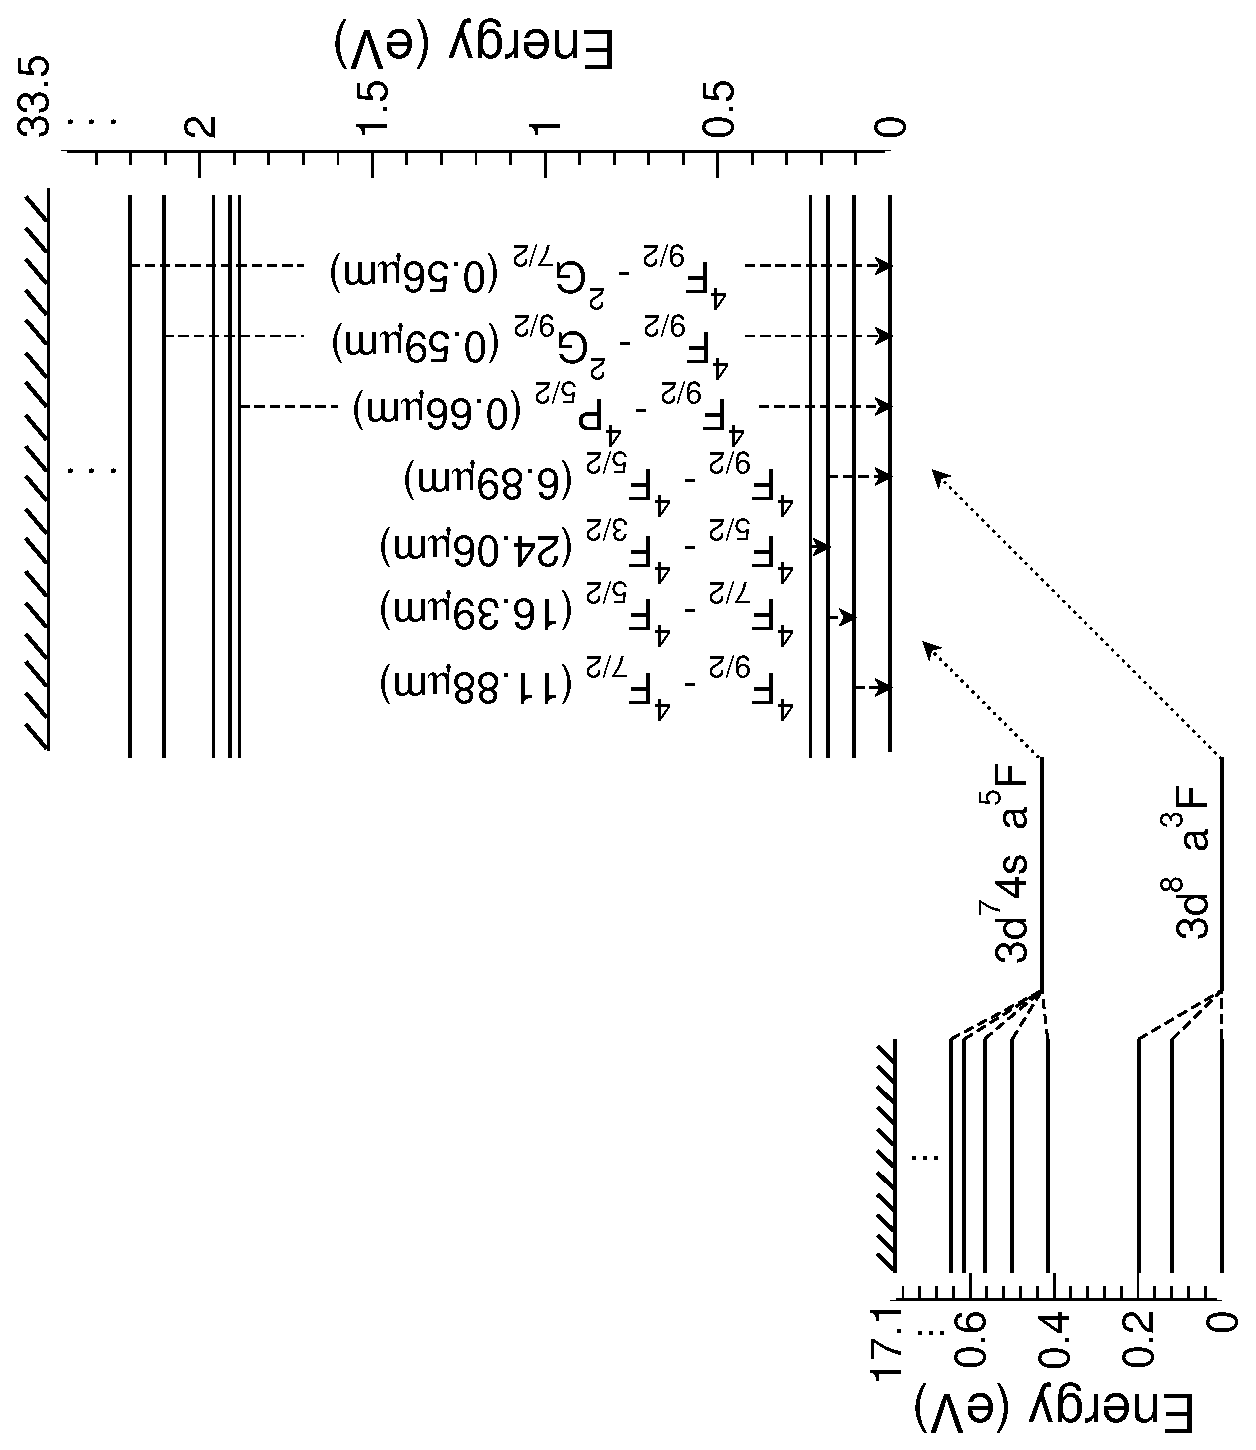
\includegraphics[scale=0.78, angle=-90]{Figures/Argon/photo/figure1.eps}
\caption{Photoionization cross-section from the initial $^2$P$^{\rm{o}}_{3/2}$ to allowed final states given in Mb on a logarithmic scale against the photon energy in eV. The dashed black line represents the result from \textit{DARC1} and the solid blue line is the contribution from levels indexed 1 - 5 in Table \ref{tab:arg_energy}. The solid red line is the extension to \textit{DARC2}. \label{fig:arg_partial}}
\end{sidewaysfigure}
%%%%
%%%
%%
%

Before embarking on the large scale \textit{DARC3} calculation we thought it prudent to investigate first the important properties and characteristics found in the photoionization cross-section of Ar$^{+}$ in its ground state. In Figure \ref{fig:arg_partial}
we present the total photoionization cross-section in Mb on a logarithmic scale as a function of photon energy in eV, from the initial ground Ar$^{+}$ $^2$P$^{\rm{o}}_{3/2}$ state to all allowed final states. Three data sets are presented in this figure; both the 209 level \textit{DARC1} and its contributions from the 3s$^2$3p$^4$ levels indexed as 1 - 5 in Table \ref{tab:arg_energy} and the extended 257 level \textit{DARC2} calculation. Clearly Figure \ref{fig:arg_partial} shows the importance of including at least the first five 3s$^2$3p$^4$ levels of Ar$^{2+}$ in this photoionization calculation. The contributions from these levels dominates the total cross-section up to a photon energy of approximately 50 eV and all three calculations exhibit excellent agreement up to this point. It is essential, therefore, that an accurate description is achieved for the wavefunction representation of those low-lying levels. Above 50 eV the additional levels associated with the more complex \textit{DARC1} and \textit{DARC2} models come into play and the cross-section rises as we move to higher photon energies as more channels become accessible. Interestingly the inclusion of the additional 3s$^2$3p$^3$4d and 3s$^2$3p$^3$5s levels in the \textit{DARC2} model has little or no effect on the photoionization cross-section produced by the \textit{DARC1} model up to 60 eV, both datasets showing near perfect agreement. Therefore we do not retain these additional 3s$^2$3p$^3$4d and 3s$^2$3p$^3$5s configurations in our largest \textit{DARC3} calculation as seen from Table \ref{tab:arg_calculations}.

%
%%
%%%
%%%%
\begin{sidewaysfigure}
\centering
    \includegraphics[scale=0.78, angle=-90]{Figures/Argon/photo/figure2_1.eps}
\caption{Total photoionization cross-section measured in Mb on a logarithmic scale as a function of photon energy in eV. All results display the initial ground state, statistically weighted $^2$P$^{\rm o}$, with $J=3/2$ and $J=1/2$ odd states to all allowed final states. A 10 meV gaussian convolution at full-width half-maximum is applied to compare directly with experimental resolution for all theoretical calculations. The yellow circles, grey circles with error bars, and solid green line are the experimental results, absolute measurements at resonance free regions and theoretical calculations respectively, performed by \citet{2011PhRvA..84a3413C}. The red dashed and blue lines represent our present \textit{PBP3} and \textit{DARC3} calculations respectively. \label{fig:arg_ground}}
\end{sidewaysfigure}
%%%%
%%%
%%
%

\subsection{Valence shell photoionization}\label{sec:arg_valence}
The only available data currently in the literature for valence shell photoionization of Ar$^{+}$ up to photon energies of 60 eV is performed by \citet{2011PhRvA..84a3413C}. In this Chapter both theoretical and experimental cross-sections are presented. Absolute cross-sections are obtained from the merged beam technique at the Advanced Light Source (ALS) with a spectral resolution of 10 meV. It was found that the primary ion beam contained a mixture of both $^2$P$_{3/2}^{\rm o}$ and $^2$P$_{1/2}^{\rm o}$ initial states. Hence the total cross-section was presented as a statistical weighting of the odd parity $J=3/2$ ground and $J=1/2$ metastable states respectively. The accompanying theoretical cross-sections presented by \citet{2011PhRvA..84a3413C} were evaluated using the semi-relativistic Breit-Pauli $R$-matrix approach. A total of 48 $LSJ\pi$ fine-structure levels were included in the wavefunction representation with configurations 3s$^2$3p$^4$, 3s3p$^5$, 3p$^6$ and 3s$^2$3p$^2$3d$^2$. Some important correlation effects are thus omitted from this model such as levels associated with the 3s$^2$3p$^3$3d configuration and those arising from the lower $n=4$ complex. 

In order to compare with this data we present in Figure \ref{fig:arg_ground} the total photoionization cross-section from the initial $^2$P$^{\rm{o}}$ ground state of Ar$^{+}$ statistically weighted to the $J=3/2$ and $J=1/2$ states. There are two of our calculations in the figure, the most sophisticated \textit{DARC3} model and, in order to perform a direct comparison with the Breit-Pauli theoretical results of \citet{2011PhRvA..84a3413C}, the \textit{PBP3} 124 level model outlined in Table \ref{tab:arg_calculations}. To match experimental resolving power, we convolute our total results with a 10 meV gaussian profile at full-width half-maximum. In addition, to replicate the target thresholds, we have shifted our threshold values recorded in Table \ref{tab:arg_energy} to the experimental NIST values where possible, during the diagonalization of the Hamiltonian matrix. The remaining levels not contained in NIST are shifted by an average proportion to each corresponding angular and spin momentum state, which has little effect on the background and is meant only for consistency. This ensures that resonance features are properly positioned with respect to the observed thresholds, making a direct comparison with experiment more meaningful.

%
%%
%%%
%%%%
\begin{sidewaysfigure}
\centering
\includegraphics[scale=0.78, angle=-90]{Figures/Argon/photo/figure2_2.eps}
\caption{Photoionization cross-section measured in Mb on a logarithmic scale as a function of the photon energy between 27.8 - 29.2 eV just above threshold. Presented is the current statistically weighted, initial ground state, \textit{DARC3} calculation against the experimental values from \citet{2011PhRvA..84a3413C} provided in Figure \ref{fig:arg_ground}. \label{fig:arg_zoom}}
\end{sidewaysfigure}
%%%%
%%%
%%
%

We can clearly see in Figure \ref{fig:arg_ground} that the low energy region just above threshold is completely dominated by 3s$^2$3p$^5$ $\rightarrow$ 3s$^2$3p$^4nl$ transitions occurring at discrete energies prior to the ejection of an electron. This densely populated region of Rydberg resonances up to approximately 30 eV is followed by a steep decline in the photoionization cross-section forming the expected Cooper minimum around 45 - 50 eV. This minimum is well known to appear in the spectra of noble gases \citep{1962PhRv..128..681C}. Above this minimum the cross-section rises due to excitations from $3p \rightarrow 3d$ transitions, before monotonically decreasing towards zero with increasing photon energy. 

Excellent agreement is evident between the 124 level \textit{PBP} and the 48 level Breit-Pauli calculation of \citet{2011PhRvA..84a3413C}, for all photon energies up to 60 eV. Note that the cross-section in Figure \ref{fig:arg_ground} is plotted on a log scale. Evidently the larger basis expansion of the present \textit{PBP} evaluation, which includes the $4s$, $4p$ and $4d$ orbitals, has minimal effect on the resulting photoionization cross-section. Both of these Breit-Pauli evaluations, however, underestimate the cross-section above roughly 45 eV and lie considerably lower than the experimental measurements from ALS. The larger \textit{DARC3} evaluation, incorporating 557 fine-structure levels, gives much better agreement with experiment at photon energies above the Cooper minimum. The additional levels included, and the Rydberg resonances converging onto their thresholds, have the effect of raising the cross-section above 45 eV.

In order to further emphasize the excellent agreement between the \textit{DARC3} and the experimental measurements, we isolate the photon energy region just above threshold, from 27.8 - 29.2 eV, in Figure \ref{fig:arg_zoom}. It is clearly evident that the disparities found between theory and experiment in this very narrow energy range are negligible and excellent conformity is achieved. This high level of agreement supports the accuracy of the \textit{DARC3} evaluation and we believe that these valence shell photoionization cross-sections for the ground state of Ar$^{+}$ accurately reproduce the experimental spectrum. 

%
%%
%%%
%%%%
\begin{figure}
\includegraphics[scale=0.55, angle=-90]{Figures/Argon/photo/figure3.eps}
\caption{Total ground state photoionization cross-section measured in Mb as a function of the photon energy between 0 - 280 eV. The transition is from the initial state 3s3p$^6$ $^2$S$_{1/2}$ to all allowed final states from the \textit{DARC3} model. \label{fig:arg_excited}}
\end{figure}
%%%%
%%%
%%
%

In Figure \ref{fig:arg_excited} we present the total photoionization cross-section for the process defined in equation (\ref{eq:rmat_totphoto}), photoionization from the lowest excited initial 3s3p$^6\; ^2$S$_{1/2}$ bound state of Ar$^{+}$ to all possible allowed final states of Ar$^{2+}$. These evaluations were carried out using the \textit{DARC3} model and present for the first time cross-sections for photoionization from an excited Ar$^{+}$ state. There are no other theoretical or experimental data with which we can compare in this figure. The cross-section is presented as a function of the photon energy in eV which ranges from just above the ionization threshold to beyond the opening of the L$_{2}$-shell thresholds. The photoionization cross-section tends towards zero with increasing energy, and it is only due to the inclusion of the additional 10 hole states in the \textit{DARC3} model do we witness contributions to the cross-section at photon energies between 200 - 250 eV. 

%
%%
%%%
%%%%
\begin{sidewaysfigure}
\centering
\includegraphics[scale=0.78, angle=-90]{Figures/Argon/ephaseplot/ephaseplot.eps}
\caption{The derivative of the eigenphase sum just above the 3s$^2$3p$^4$ $^1$D$_2$ threshold as function of photon energy in eV. The solid black curve are the 3s$^2$3p$^4(^1$S$_0)ns$ $^2$S$_{1/2}$ resonant states, the dashed curve is for 3s$^2$3p$^4(^1$S$_0)ns$ $^2$D$_{3/2}$ and the dotted curve are the 3s$^2$3p$^4(^1$S$_0)ns$ $^2$D$_{5/2}$ even resonant states. The corresponding photoionization cross-section from the initial statistically weighted $^2$P$^{\rm{o}}$ to allowed final states in Mb is presented on the lower graph also as a function of photon energy in eV. \label{fig:arg_ephase}}
\end{sidewaysfigure}
%%%%
%%%
%%
%

It can be see  from Figure \ref{fig:arg_ephase}, just above the 3s$^2$3p$^4$ $^1$D$_2$ threshold, that the resonances are well isolated. We can therefore implement the $QB$ technique again as described in Section \ref{sec:rmat_qb} to identify these resonances. We provide the eigenphase sum derivate calculated from equation (\ref{eq:rmat_ephasesum}) in Figure \ref{fig:arg_ephase} to show how the steep rise indicates the presence of a resonant state. They can easily be identified as 3s$^2$3p$^4(^1$S$_0)ns$ $^2$S$_{1/2}$ (solid curve), 3s$^2$3p$^4(^1$S$_0)ns$ $^2$D$_{3/2}$ (dashed curve), and 3s$^2$3p$^4(^1$S$_0)ns$ $^2$D$_{5/2}$ (dotted curve). Since the outer $nl$ electron couples with a singlet state, we are able to assign each an $LS\pi$ state. The linewidths are then calculated from the eigenphase sum as in equation (\ref{eq:rmat_qbwidth}). The general trend of the linewidths for the three $J\pi$ resonant states can be visualized in Figure \ref{fig:arg_linewidths}. We have used the photoionization cross-section from the \textit{PBP3} model in these plots as we encounter problems with the large close-coupling wavefunction expansion in the \textit{DARC3} model. The {\sc qb} codes have not been parallelized, and this limits the feasibility to perform a thorough analysis with these large calculations. 


% FIGURE %
%%%%%%%%%%%
%%%%%%%%%%%
\begin{figure}
\includegraphics[scale=0.65, angle=-90]{Figures/Argon/ephaseplot/linewidth.eps}
\caption{Linewidths, $\Gamma$ in meV presented as a function of energy in eV for increasing $n$ in each $nl$ Rydberg series. a) represents the 3s$^2$3p$^4(^1$S$_0)ns$ $^2$D$_{5/2}$, b) 3s$^2$3p$^4(^1$S$_0)ns$ $^2$D$_{3/2}$, and c) 3s$^2$3p$^4(^1$S$_0)ns$ $^2$S$_{1/2}$ resonant states. \label{fig:arg_linewidths}}
\end{figure}

\subsection{L$_{2}$-shell photoionization}\label{sec:arg_lshell}
Calculations and experiment have been carried out at the L$_{2}$-shell energy region between 250 - 280 eV by \citet{2012PhRvA..85d3408B} at the SOLEIL facility in France as described in Section \ref{sec:arg_introduction}. All the results herein have been convoluted with a 140 meV Gaussian profile at full-width half-maximum to match the spectral resolution of experiment. Similar to the valence shell comparisons, the initial ground state cross-section is formed from a statistically weighted average of the contributions from the odd $J=3/2$ and $J=1/2$ partial waves. Due to time of flight between the ion source and interacting region, excited levels can populate the main ion beam. This leads to a possible inclusion of the initial 3s3p$^6$ $^2$S$_{1/2}$ bound state which may also contribute to the total cross-section. In Figure \ref{fig:arg_excited} we have already shown the immediate result of the lowest excited initial bound state transitions arising from the configuration 3s3p$^6$.

In order to compare with experiment, we have presented our results against various ionization channels from \citet{2012PhRvA..85d3408B} in Figure \ref{fig:arg_l-shell}. The timescale for Auger decay is much shorter than the time of flight required by the Argon ions after interaction with a photon, and therefore, the single ionization channel from experiment depicts the characteristics of photoionizing a valence electron. We can directly compare with this process in Figure \ref{fig:arg_l-shell} by omitting the contribution from the additional 10 target states annotated by asterisks. Both above and during these thresholds we expect a rise in the photoionization cross-section as more channels are opened and become accessible. The total result obtained by \textit{DARC3} can be compared directly to the combination of both single and double ionization modes of experiment. We have neglected the error bars for both modes in order to visualise the results more clearly.

%
%%
%%%
%%%%
\begin{sidewaysfigure}
\centering
\includegraphics[scale=0.78, angle=-90]{Figures/Argon/gt270.eps}
\caption{The photoionization cross-section is presented against the photon energy in eV above 261.2 eV. The solid black line represents our current \textit{DARC3} model convoluted at 140 meV full-width half-maximum and the dashed black line is the contribution to the cross-section from valence shell photoionization of the 3s and 3p. The blue circles are experimental values of \citet{2012PhRvA..85d3408B} for the single ionization channel and pink circles represent the total contribution. \label{fig:arg_l-shell}}
\end{sidewaysfigure}
%%%%
%%%
%%
%

We now present in Figure \ref{fig:arg_l-shell-big} a) the photoionization cross-section, this time on a linear scale, as a function of incident photon energy in eV across the L$_{2}$-shell threshold range from 250 - 270 eV. Comparisons are made between the present \textit{DARC3} cross-section and the measurements performed by \citet{2012PhRvA..85d3408B}. Clearly excellent agreement is evident between theory and experiment across the range considered, as the features and energy positions of the resonance profiles exhibit good agreement. We note that as we have employed orbitals optimized on the valence state photoionization, an energy shift of 7.5 eV was required to match the experimental spectra to our current results. The theory clearly predicts this process to a high standard of accuracy and allows us to benchmark the quality of results obtained from experiment. We have also provided comparisons in Figure \ref{fig:arg_l-shell-big} b) and c) with {\sc mchf} and {\sc opas} calculations also performed by \citet{2012PhRvA..85d3408B}. The agreement does not seem to match to the same degree of accuracy, but similarities are clearly present. The magnitudes are similar, but the positions of the resonant states are often misaligned by several eV. This asserts the $R$-matrix technique again as it provides excellent agreement with experimental results.

% FIGURE %
%%%%%%%%%%%
%%%%%%%%%%%
\begin{figure}
    \centering
    \begin{subfigure}[b]{0.9\textwidth}
\includegraphics[scale=0.5, angle=-90]{Figures/Argon/l-shell/expt.eps}
        \caption{\textit{DARC3} vs. Experiment}
        \label{subfig:arg_7}
    \end{subfigure}
    ~ %add desired spacing between images, e. g. ~, \quad, \qquad, \hfill etc. 
      %(or a blank line to force the subfigure onto a new line)
    \\
    \begin{subfigure}[b]{0.9\textwidth}
\includegraphics[scale=0.5, angle=-90]{Figures/Argon/l-shell/mcdf.eps}
        \caption{\textit{DARC3} vs. {\sc mchf}}
        \label{subfig:arg_8}
    \end{subfigure}
    ~ %add desired spacing between images, e. g. ~, \quad, \qquad, \hfill etc. 
    %(or a blank line to force the subfigure onto a new line)
    \\
        \begin{subfigure}[b]{0.9\textwidth}
\includegraphics[scale=0.5, angle=-90]{Figures/Argon/l-shell/opas2.eps}
        \caption{\textit{DARC3} vs. {\sc opas}}
        \label{subfig:arg_9}
    \end{subfigure}
    ~ %add desired spacing between images, e. g. ~, \quad, \qquad, \hfill etc. 
      %(or a blank line to force the subfigure onto a new line)
    \caption{Photoionization cross-section measured in Mb as a function of the photon energy in eV between 248 - 272 eV. The solid black curve corresponds to our current \textit{DARC3} model for the statistically weighted initial $^2$P$^{{\rm o}}$ state as in equation (\ref{eq:arg_photo1}), convoluted at 140 meV full-width half-maximum, for all three subfigures. Subfigure a) is the experimental results, b) is the {\sc mchf} calculation and c) is the {\sc opas} calculation all performed by \citet{2012PhRvA..85d3408B}. \label{fig:arg_l-shell-big}}
\end{figure}

In an attempt to investigate the features further, we have broken down the spectrum in Figure \ref{fig:arg_l-shell-resonance} from the total into each of the allowed, final, even $J$ states $J=1/2$, $J=3/2$ and $J=5/2$. Clearly visible is the intense spike at $\approx 254.9$ eV which is dominated by transitions of the form, $2p$ $\rightarrow$ $nd$, $ns$ which are engulfed by the convolution. The second strong peak at $\approx 255.65$ eV is visible mostly through the metastable initial state transition from another strong $2p$ $\rightarrow$ $nd$, $J = 3/2$ resonance. In reference to Figure \ref{fig:arg_excited}, the cross-section has already reached close to zero in the photon energy range of interest and therefore any contribution to the total cross-section from these initial excited bound states would result in a reduction to the intensity of each resonant state. 

% FIGURE %
%%%%%%%%%%%
%%%%%%%%%%%
\begin{figure}
\centering
\includegraphics[scale=0.80, angle=-90]{Figures/Argon/resonances.eps}
\caption{The total convoluted 140 meV at full-width half-maximum photoionization cross-section between 254 - 256 eV taken from Figure \ref{fig:arg_l-shell-big} highlighting the intense resonant peaks. The spectra is broken into the contributions from each dipole allowed symmetry from both initial (middle third) and metastable (bottom third) initial states according to their statistical weighting. The total (top third) summed contribution is presented by the solid black curve and the two dominate resonances are marked by the dashed line. \label{fig:arg_l-shell-resonance}}
\end{figure}

This method of deconstructing the cross-section is also important to identify which initial state has been photoionized during the experiment. It is clear however that the strongest profiles are not well isolated and therefore eliminates the possibility to further conduct any analysis on the weighted contributions. We therefore retain the statistical averaging of the ground state as our best result.

The overlapping nature of the resonant states makes it difficult to accurately evaluate resonance widths and assign each transition taking place. It is possible to deduce that the hole resonant states arise from $2p$ $\rightarrow$ $nd$, $(n+1)s$ transitions for $n\ge3$, and correspond to the strongest peaks evident in Figure \ref{fig:arg_l-shell-resonance}.

%%%%%%%%%%%%%%%%%%%%%%%%%%
%%%%%%%%%%%%%%%%%%%%%%%%%%
%%%%%%%%%%%%%%%%%%%%%%%%%%
%%%%%%%%%%%%%%%%%%%%%%%%%%
% END RESULTS %

% CONCLUSIONS %
%%%%%%%%%%%%%%%%%%%%%%%%%%
%%%%%%%%%%%%%%%%%%%%%%%%%%
%%%%%%%%%%%%%%%%%%%%%%%%%%
%%%%%%%%%%%%%%%%%%%%%%%%%%

\section{Conclusions}\label{sec:arg_conclusions}
In this Chapter we have invested our time towards obtaining an accurate target state representation for Ar$^{2+}$. We have focused on six possible models in total, using two different forms for the total energy operator as defined in equation (\ref{eq:many_hbp}) and equation (\ref{eq:many_dirac_ham}). The models \textit{PBP1-3} have been optimized using the computer package of {\sc civ3} by including the Breit-Pauli operators as one body corrections to the non-relativistic Hamiltonian. On the other hand, \textit{DARC1-3} avails of the Dirac-Coulomb Hamiltonian as defined in equation (\ref{eq:many_dirac_ham}). 

We first investigate the importance of configuration interaction required in the \textit{PBP} models. For this we directly compare the length and velocity forms for the oscillator strengths, and note the improvement between \textit{PBP1} and \textit{PBP3}. We have also compared out work with two other theoretical approaches from \citet{2006ADNDT..92..607F} and \citet{2001JQSRT..69..171L} with similar agreement achieved. The energy eigenvalues from the target states also compare well with the current NIST data provided by \citet{2010JPCRD..39c3101S} and two other theoretical $R$-matrix calculations performed by \citet{2012EPJD...66...84S} and \citet{2009A&A...500.1253M} in Table \ref{tab:arg_energy}.

Photoionization cross-sections have been produced for the three lowest states of Ar$^{+}$ from these two independent $R$-matrix methods, {\sc darc} and {\sc bp} for select models. Both evaluations differ considerably in size and sophistication as we have summarized into Table \ref{tab:arg_calculations}. All photoionization spectra reported in this paper have been properly resolved with a very fine mesh of incident photon energies and comparisons have been made where possible. To exhibit the nature of the nature of the linewidths in the $nl$ Rydberg series of resonances, we have provided the eigenphase sum derivative and linewidths for three well isolated series above the 3s$^2$3p$^4$ $^1$D$_2$ threshold. There is also good agreement here with the comparison with linewidths from \citet{2011PhRvA..84a3413C} with our \textit{PBP3} model.

Excellent agreement is clearly evident between theory and experiment up to the L$_{2}$-shell energy region for all photon energies considered. Agreement has been obtained with the present \textit{DARC3} model which was shown to better reproduce experimental measurements for a number of energy ranges, particularly just above threshold and the Cooper minimum in the low energy section of the spectrum. The results pertaining to the energy region of 250 - 270 eV are the first $R$-matrix calculations performed to date and clearly resolve the majority of resonance structure. This model thus represents the largest and most sophisticated evaluation of Ar$^{+}$ photoionization from the ground and first excited state, providing the most complete cross-sections.

%---------------------------------------------------------------------------------------



% FIGURE %
%%%%%%%%%%%
%%%%%%%%%%%
%\begin{figure}
%\includegraphics[scale=0.53, angle=-90]{Figures/Argon/Oscillator_compare/new_all.eps}
%\caption{Photoionization cross-section from the initial $^2$P$^{\rm{o}}_{3/2}$ to allowed final states given in Mb on a logarithmic scale against the photon energy in eV. The dashed black line represents the result from \textit{DARC1} and the solid blue line is the contribution from levels indexed 1 - 5 in Table \ref{tab:energy}. The solid orange line is the extension to \textit{DARC2}. \label{fig:comparison}}
%\end{figure}



%There is, however, a further benefit to incorporating the 3s3p$^3$3d$^2$ states in our wavefunction expansion of the Ar III ion as it allows us to extend our evaluations to L$_{2}$-shell photoionization. 
%which results in the $\%$ difference from NIST across the lowest 29 levels from 3.613$\%$ to 2.466$\%$. Due to the inclusion of these additional levels, the present GRASP0 calculation thus increases from 209 levels to 547 levels. However, these effects are extremely important in the photoionization spectra for a true representation of these low lying wavefunctions.




